%%%%%%%%%%%%%%%%%%%%%%%%%%%%%%%%%%%%%%%%%
% Simple Sectioned Essay Template
% LaTeX Template
%
% This template has been downloaded from:
% http://www.latextemplates.com
%
% Note:
% The \lipsum[#] commands throughout this template generate dummy text
% to fill the template out. These commands should all be removed when 
% writing essay content.
%
%%%%%%%%%%%%%%%%%%%%%%%%%%%%%%%%%%%%%%%%%

%----------------------------------------------------------------------------------------
%	PACKAGES AND OTHER DOCUMENT CONFIGURATIONS
%----------------------------------------------------------------------------------------

\documentclass[12pt,usenames,dvipsnames]{article} % Default font size is 12pt, it can be changed here

\usepackage{geometry} % Required to change the page size to A4
\geometry{a4paper} % Set the page size to be A4 as opposed to the default US Letter

\usepackage{graphicx} % Required for including pictures

\usepackage{float} % Allows putting an [H] in \begin{figure} to specify the exact location of the figure
\usepackage{wrapfig} % Allows in-line images such as the example fish picture

\usepackage{lipsum} % Used for inserting dummy 'Lorem ipsum' text into the template

\usepackage{hyperref}

\usepackage{gantt}
\usepackage{pdflscape}
\usepackage{pdfpages}
\usepackage{setspace}
\linespread{1.2} % Line spacing

%\setlength\parindent{0pt} % Uncomment to remove all indentation from paragraphs

\graphicspath{{Pictures/}} % Specifies the directory where pictures are stored

\setcounter{secnumdepth}{4}
\setcounter{tocdepth}{4}
%======================================================================================
%      EXTRA PREAMBLE INCLUSIONS
%======================================================================================

%--------------------------------------------------------------------------------------
%       CODE SNIPPETS
%--------------------------------------------s------------------------------------------

\usepackage{listings} % Required for inserting code snippets
%\usepackage[usenames,dvipsnames]{color} % Required for specifying custom colors and referring to colors by name

\definecolor{DarkGreen}{rgb}{0.0,0.4,0.0} % Comment color
\definecolor{highlight}{RGB}{250,220,150} % Code highlight color

\lstdefinestyle{Style1}{ % Define a style for your code snippet, multiple definitions can be made if, for example, you wish to insert multiple code snippets using different programming languages into one document
language=C++, % Detects keywords, comments, strings, functions, etc for the language specified
backgroundcolor=\color{highlight}, % Set the background color for the snippet - useful for highlighting
basicstyle=\footnotesize\ttfamily, % The default font size and style of the code
aboveskip={-40ex},
breakatwhitespace=false, % If true, only allows line breaks at white space
breaklines=true, % Automatic line breaking (prevents code from protruding outside the box)
captionpos=b, % Sets the caption position: b for bottom; t for top
commentstyle=\usefont{T1}{pcr}{m}{sl}\color{DarkGreen}, % Style of comments within the code - dark green courier font
deletekeywords={}, % If you want to delete any keywords from the current language separate them by commas
%escapeinside={\%}, % This allows you to escape to LaTeX using the character in the bracket
firstnumber=1, % Line numbers begin at line 1
frame=single, % Frame around the code box, value can be: none, leftline, topline, bottomline, lines, single, shadowbox
frameround=, % Rounds the corners of the frame for the top left, top right, bottom left and bottom right positions
keywordstyle=\color{Blue}\bf, % Functions are bold and blue
morekeywords={}, % Add any functions no included by default here separated by commas
numbers=left, % Location of line numbers, can take the values of: none, left, right
numbersep=1.2em, % Distance of line numbers from the code box
numberstyle=\tiny\color{Gray}, % Style used for line numbers
rulecolor=\color{black}, % Frame border color
showstringspaces=false, % Don't put marks in string spaces
showtabs=false, % Display tabs in the code as lines
stepnumber=1, % The step distance between line numbers, i.e. how often will lines be numbered
stringstyle=\color{Purple}, % Strings are purple
tabsize=2, % Number of spaces per tab in the code
}


% Create a command to cleanly insert a snippet with the style above anywhere in the document
%\newcommand{\insertcode}[2]{\begin{itemize}\item[]\lstinputlisting[caption=#2,label=#1,style=Style1]{#1}\end{itemize}} % The first argument is the script location/filename and the second is a caption for the listing

%%%%% EXAMPLE USE CASE %%%%%
% The first argument is the script location/filename and the second is a caption for the listing

% \insertcode{"Scripts/example.pl"}{Nena would be proud.} 

%----------------------------------------------------------------------------------------


\definecolor{dkgreen}{rgb}{0,0.6,0}
\definecolor{gray}{rgb}{0.5,0.5,0.5}
\definecolor{mauve}{rgb}{0.58,0,0.82}

\lstset{frame=tb,
  language=c++,
  aboveskip=3mm,
  belowskip=3mm,
  showstringspaces=false,
  columns=flexible,
  basicstyle=\linespread{0.8}\footnotesize\ttfamily,
  %basicstyle={\small\ttfamily},
  numbers=left,
  numberstyle=\tiny\color{gray},
  keywordstyle=\color{blue},
  commentstyle=\color{dkgreen},
  stringstyle=\color{mauve},
  breaklines=true,
  breakatwhitespace=false,
  tabsize=2
}

% MY MACROS
\newcommand{\includegraphicscaption}[2]{
    \begin{figure}[h]
    \includegraphics[width=\textwidth]{#1}
    \caption{#2}
\end{figure}
}



\begin{document}

%----------------------------------------------------------------------------------------
%	TITLE PAGE
%----------------------------------------------------------------------------------------

\begin{titlepage}

\newcommand{\HRule}{\rule{\linewidth}{0.5mm}} % Defines a new command for the horizontal lines, change thickness here

\center % Center everything on the page

\textsc{\LARGE Monash University}\\[1.5cm] % Name of your university/college
\textsc{\Large Electrical Engineering}\\[0.5cm] % Major heading such as course name
\textsc{\large Final Year Project (ECE4093)}\\[0.5cm] % Minor heading such as course title

\HRule \\[0.4cm]
{ \huge \bfseries Final Report}\\[0.4cm] % Title of your document
\HRule \\[1.5cm]

\begin{minipage}{0.4\textwidth}
\begin{flushleft} \large
\emph{Author:}\\
James \textsc{Anastasiou}\\ % Your name
\emph{ID:} 23438940
\end{flushleft}
\end{minipage}
~
\begin{minipage}{0.4\textwidth}
\begin{flushright} \large
\emph{Supervisor:} \\
Dr. David \textsc{Boland} % Supervisor's Name
\\
\end{flushright}
\end{minipage}\\[4cm]

{\large \today}\\[3cm] % Date, change the \today to a set date if you want to be precise

%
\includegraphics[width=8cm]{./Pictures/Logo.eps}\\[1cm] % Include a department/university logo - this will require the graphicx package

\vfill % Fill the rest of the page with whitespace

\end{titlepage}

%----------------------------------------------------------------------------------------
%	TABLE OF CONTENTS
%----------------------------------------------------------------------------------------

\tableofcontents % Include a table of contents

\newpage % Begins the essay on a new page instead of on the same page as the table of contents 

%----------------------------------------------------------------------------------------
%       CONTENT	
%----------------------------------------------------------------------------------------
%!TEX root = ./main.tex
%----------------------
%   Significant Contribution
%----------------------

\section{Significant Contribution}

\begin{itemize}
\item Designed and implemented a Static Analysis tool for identifying potential parallelism in sequential C code.
\item Designed and implemented an AST Matcher Combinator header only library.
\item Designed and implemented a CPU and GPU benchmarking suite.
\item Designed and implemented a Templated Typeclass interface for parallel primitives in CUDA C++.
\end{itemize}

\pagebreak

%!TEX root = ./main.tex
%----------------------------------------------------------------------------------------
%	INTRODUCTION
%----------------------------------------------------------------------------------------

\section{Introduction} % Major section


%------------------------------------------------

\subsection{Purpose and Scope} % Sub-section

This document aims to provide a framework which describes the process by which my final year project will be completed, and by extension the re-evaluation of goals initially set forth in the requirements specification. In order to best achieve this aim, this document includes:

\begin{itemize}
\item Project Description
\item Re-evaluation of the inital goals
\item Project Status Overview
\item Current Position Review 
\item Timeline to Expected Completion
\end{itemize}


\pagebreak

%!TEX root = ./main.tex
%---------------------------------------------------------------------------------------- PROJECT
%DESCRIPTION
%----------------------------------------------------------------------------------------

\section{Project Description} 
My final year project aimed to create a set of tools for static analytics to help determine which
algorithms within a code-base may be easily parallelized. The specific intention of it is to provide
users with a report describing which parts of their code-base may see a potential speed-up from
redeveloping them as CUDA (GPU)\cite{cuda} kernels. In order to achieve this both benchmarking and
theoretical analysis was required, as well as static analysis of the C description of the algorithm
itself. My final project utilised a combined strategy of static AST analysis, via a hook into the
Clang compiler, as well as integration with a benchmarking suite I created that utilised real high
performance libraries for both Host and Device code. The use case of this software is for developers
working primarily in modelling and mathematically intensive areas, as these tend to provide
significant opportunity to provide improvement. The expectation of potential users is that they will
note that the report alerts them to potential speedups, and then use the performance metrics to
determine whether or not to hire a specialised engineer to redesign the relevant components of their
system.

\subsection{Compiler Analytics} 
Given a C description of an algorithm, a report is to be generated, highlighting areas within the
code that may see a potential speed-up based on matching to known GPU performant patterns. In order
to achieve this, a static analysis methodology was invoked. Direct source code analysis is
incredibly difficult, and suffers from a number of drawbacks, including the difficulty to parse C
and (notoriously difficult) C++. Considering the time constraints involved it was decided that the
analysis tool would hook into the Clang Libtooling library, which provides access to the Clang
Abstract Syntax Tree, giving a semi-syntax invariant canvas from which to identify relevant parallel
patterns.

Given the difficulty of setting up a generic build environment for the Clang tooling, I decided to
fork a project named OCLint\cite{oclint}, a C, C++ and Obj-C static analysis tool that I had worked
with earlier.  This tool provides a light framework around the Clang tooling, however most
importantly it provides sophisticated build scripts which work on a variety of operating systems and
distributions.

\subsubsection{OCLint Modification} 
Forking the OCLint project, which is licensed under a modified BSD license has saved significant
time and effort from being wasted developing a generic build system around the Clang tooling. The
OCLint software provides a direct method for interacting with the Clang AST by exposing the Clang
Libtooling headers. This increased flexibility has in turn allowed for more time to be spent
developing methods to identify parallel patterns within the generated AST. All changes to the OCLint
software are unrelated to its original intention and design, and as such no pull requests were
lodged, and no modifications I have written have moved upstream. As I have substantially
re-engineered and re-purposed the OCLint software I have elected to give it a new name, the C
Algorithm Parallelisation Analyser (CAPA).

\subsection{GPU Benchmarking}
In order to best provide theoretical performance improvements of algorithms within a codebase, an
analysis of the current hardware available is significantly important. As such rather than just
provide purely theoretical numbers, part of this project involved developing a simple set of GPU
benchmarks which seek to show performance metrics for the identified patterns within the code
analyser. This in effect means that reports generated by the analytics tool may contain specific
information pertaining to the hardware available on the current build and test system. In order to
achieve the best outcome, CUDA was decided on as the framework for development.

\subsubsection{Benchmarks}
GPUs are exceptionally good at high throughput calculations, one particular example is SIMD, meaning
\emph{Same Instruction Multiple Data}. The performance of GPUs and the algorithms they are
particularly useful for is well under continual research, however general problem classes that GPUs
are able to solve efficiently are well understood. These problem sets include algorithms that can be
described by any of the following:

\begin{itemize} 
    \item Map 
    \item Fold/Reduce 
    \item Scan/Prefix Network 
    \item Matrix Operations
\end{itemize}

The actual speed improvements derived from redeveloping serial code to take advantage of the
massively parallel compute power of a GPU differs between each of these operations, however many
serial algorithms have equivalent or more performant alternate parallel implementations. As such
this project involves developing a small set of benchmarks for GPUs that determine their
performance in each of these categories. In order to satisfy time constraints and recognise real
world concerns, I elected to use existing optimised libraries for the individual components of the
benchmarking. I relied on the Eigen library\cite{eigen} for host side matrix operations. On the
device side I relied on a combination of the Thrust template library\cite{thrust} in combination
with CuBLAS\cite{cublas}

\subsubsection{CUDA} 
CUDA is Nvidia's proprietary library and toolchain for developing parallel software. There are 2
main frameworks in the GPU programming space, CUDA and OpenCL. Whilst OpenCL is a FOSS platform, the
development tools are severely lacking in comparison to the CUDA toolkit, and as such it was an easy
decision to follow through with the CUDA. This however has limited the performance metrics to only
comparisons involving CUDA enabled graphics cards. This is not too great a concern however, as the
benchmarking module is highly extensible and as a result can easily integrate with a variety of
backends, including OpenCL or OpenMP.

\pagebreak

%!TEX root =./main.tex -------------------------------- LITERATURE REVIEW
%--------------------------------

\section{Literature Review} 
\subsection{Introduction}
Optimisation and computational efficiency are two pillars of good program design, much research has
been undertaken in the search of improving performance and extracting hardware maximum efficiency.
Although the current literature covers an extensive range of research, this review seeks to focus
primarily on the topics of automatic vectorisation, alternative hardware (GPU/FPGA) performance in
parallel contexts, and finally the utilisation of Static Analysis and Profiling to assist in the
process of identifying potential optimisation in the massively parallel computation paradigm.
Individually these are all large topics of research, and as such this review will be focusing
primarily on computational performance, rather than power consumption or algorithm efficiency. The
purpose of this review is to provide a contextualisation around my final year project, in order to
identify potential challenges in the problem space, as elucidated by prior research. 

\subsection{Automatic Vectorisation}
Automatic vectorisation is a tool employed by many compiler designers in order to generate ASM which
utilises specialised hardware level vector instructions.  Same Instruction Multiple Data (SIMD)
instructions seek to process multiple elements of a dataset simultaneously, utilising multiple
processing units in order to achieve data level parallelism. Roger Espasa and Mateo Valero
\cite{espasa1997exploiting} explore the potential benefits of Data-Level Parallelism by
investigating computer architectures to utilise both Instruction Level and Data Level parallel
constructs. Within their research they identify and develop an architecture to utilise SIMD
instructions to leverage the performance benefits, clearly demonstrating the performance improvement
this parallel strategy provides. These techniques have since been further developed by Compiler
designers, with the LLVM/Clang team employing two forms of automatic vectorisation within their
optimising C compiler \cite{website:llvmAutoVectorize}. The Clang team focused on developing Loop
Level Vectorisation and Super Word Level Vectorisation in order to leverage parallelisation in the
target architecture.  Their automatic loop vectoriser is capable of providing an increase in
processing speed of 3 times, when tuned specifically for the Intel Core-i7 AVX instruction set. This
is a clear demonstration of the benefits already being seen by optimising compilers manipulating
sequential programs into those which leverage the power of parallel computation. The LLVM optimiser
however has some flaws which are identified by Yulei Sui, Xiaokang Fan, Hao Zhou, and Jingling Xue
who developed Loop-oriented array and field sensitive Pointer Analysis (LPA) in order to combat the
suboptimal performance of the LLVM auto-vectoriser \cite{sui2016loop}. The authors identified alias
analysis as being a potential cause of the LLVM compiler missing optimisation opportunities. They
created an analysis framework around both flow-insensitive and flow-sensitive pointer construct. By
hooking into the LLVM’s partial SSA form they exploited the reduced semantic complexity to
algorithmically generate superior memory patterns, and by extension developed a superior loop
vectoriser, with performance up to 10\% better than the original LLVM. This research again
demonstrates the performance opportunities created by parallel computation, however they are all
fundamentally limited by the CPU’s capacity to perform SIMD operations. Most CPU architectures have
at most 8 complex computing cores, limiting the maximum potential throughput, however GPU
architectures have the capacity for massively parallel computation. The typical design inherently
leverage SIMD concepts containing thousands of simple computational cores with high memory
bandwidth. Thus whilst automatic vectorisation has substantial performance potential, most current
literature is focused on continuing to improve computational efficiency of host bound programs,
rather than looking towards exploiting the massively parallel computational power of modern GPU’s.

\subsection{Parallelism}
General Purpose GPU programming seeks to exploit the parallel performance characteristics of the GPU
architecture; identification and development of algorithms which leverage this design pattern can
provide substantial computational speedups. The authors of \cite{papadrakakis2011new} explore the
fundamentals of GPGPU programming, and the CUDA architecture. Inherent within the CUDA architecture
is hybrid CPU-GPU programming to produce the most efficient solution. In the example described the
authors extract maximum parallelism from Matrix operations, and leave complex control flow to the
CPU, thus developing a solution which maximises the performance of the individual components of the
Hybrid Host-Device model. The proposed solution utilises parallel primitives such as the Reduction,
which exploits parallelism by utilising a summation tree. This requires that the data and binary
operator form a semigroup (The set of data must be closed under an associative binary operator). In
their example the set is of integers, and the operator is addition, which holds these properties.
The concept of parallel primitive operations is further expanded by \cite{nagarajan2011accelerating}
which provides terminology to describe parallel patterns for both computation and communication.
Although this research focuses on parallelism within FPGA’s the primitive operations are examples of
fundamentally parallel operations, exposing high levels of optimisation potential through SIMD
data-paths. The authors look to extract performance from their FPGA implementation of potentially
parallelisable algorithms; their key focus is on the Parzen window technique of Gaussian PDF
estimation, as well as K-Means clustering. From their research they develop a concept of
pattern-based algorithm decomposition; as a means of exposing potential parallelism within a
codebase to individuals with little or no experience with highly parallel code.  The authors
describe a limitation in the existing development framework, where FPGA based systems are developed
on by only highly specialised and skilled developers. This concept is explored by the authors of
\cite{sengupta2007scan} in which they describe the limitation upon many programmers is
the lack of a breadth of libraries which exploit the benefits of GPGPU programming.  Within this
paper they present the problem of fragmentation within the GPU programming space, with competing
standards and API’s resulting in specialists rolling their own solutions to many problems, resulting
in minimal code re-use. The current solution to the code reuse problem is the introduction of
parallel algorithms within the C++ STL as well as CUDA based libraries such as CuBLAS and Thrust,
which aim to provide programmers with a foundation from which to build larger programs, without
being forced into having a full understanding of programming on a GPU. Given the power and
performance characteristics of GPU’s there is a great incentive to move computationally expensive
algorithms onto these devices, currently however there are many roadblocks preventing individuals
and organisations from exploiting the potential improvements within their codebase, the high barrier
to entry can be difficult to overcome, especially with the limited capabilities of identifying how
beneficial any redevelopment may actually be.

\subsection{Static Analysis}
Static Analysis is the analysis of the original source statements of a program, it provides a method
by which the semantics of a program may be identified.  Typically, Static Analysis is utilised in
order to identify bugs within a codebase \cite{bessey2010few}, there is a litany of literature which
describes a variety of processes through which one can employ Static Analysis to search out and find
bugs \cite{ball2001automatically} \cite{bush2000static}. These tools rely on parsing the source of a
program and identifying the anti-patterns within, alerting developers to their potential mistakes.
Additionally, many static analysers provide complexity statistics about the analysed source; it is
often the intention of static analysers to provide the developer with a summary of information about
their codebase which facilitates further investigation and development.  Although there has been a
large amount of research into static analysis for the purpose of detecting and eliminating bugs,
there is a lack of research into the topic of utilising static analysis for the purpose of
performance improvements.  Static analysis as a tool is rarely used to facilitate optimisation
improvements within a codebase; programmers often utilise profiling in order to determine where to
invest development time focused on optimisation.  Clearly this presents a divide, where programmers
often utilise Static Analysis and Profiling in a competing demands structure for developer time.
Within the NVidia High-Productivity CUDA Programming presentation \cite{nvidiapresentation}
they recommend the utilisation of a process called “APOD” Assess-Parallelise-Optimise-Deploy.
Within the Assessment and Optimisation phase of the process they recommend utilising profilers in
order to make determinations about what aspect of the code requires further development. The
weakness of profiling however is that it is often very time consuming, additionally it requires an
individual developer have an understanding of how to potentially translate sequential serial
algorithms into their massively parallel equivalents. 
 
\subsection{Summary}
TODO:

\pagebreak

%!TEX root = ./main.tex
%----------------------------------------------------------------------------------------
% PARALLEL COMPUTATION
%----------------------------------------------------------------------------------------

\section{Parallel Computation} % Major section
Parallel computing is a type of computation whereby many operations are performed simultaneously, as
opposed to serial computing where only one operation occurs at a time\cite{wikiRef1}. Parallel
computing has been used as a high performance computing technique for some time, with recent
physical limitations on serial processors forcing further development in the parallel world.  Modern
parallel computing focuses primarily on extracting maximum performance from data level parallelism,
the process by which independent processors act on a distributed load of data, often performing SIMD
(Signle Instruction Multiple Data) operations. 

\subsection{SIMD}
SIMD describes a computation structure by which many processing units execute the same instruction
on multiple data in parallel. SIMD allows for significant computation speed improvements over
traditional serial data processing by operating on multiple data at once. The theoretical speed
improvements a SIMD processor has over a traditional serial processor can be described by: $ speedup
\propto min\left(N_{processing\_units}, N_{data}\right) $. In many computing environments $N_{data}$
is significantly larger than $N_{processing\_units}$ simplifying the relationship to merely $
speedup \propto N_{processing\_units}$. Thus it is clear that with increasing number of processing
units the commputation speed increases. As a result of this relationship devices have been developed
which can exploit this fact, most modern CPU's include some form of Vectorised SIMD instruction set.
Advanced Vector Extensions (AVX) are an extension to the x86 instruction set which are supported by
both AMD and Intel, which utilises SIMD to improve processor performance for highly parallel
workloads. GPU's however are far more suited to the task of performing SIMD operations as they often
have orders of magnitude more processing units than comporable CPU's.

\subsection{Parallel Limitations} 
One of the largest limitations that concerns parallel computing is data dependency. A data
dependency is a situation where operations in the algorithm require data from earlier in the
algorithm in order to continue processing. An example situation would be:
\lstinputlisting{./Code/DataDependency.cpp} in this case we have two examples of data dependency, in
the first case we are trying to normalise the vector by subtracting the mean. This is an example of
a data dependency where a SIMD operation relies on prior information, in this case this will not
impact our ability to perform the operations simultaneously, as at no point does the input
information rely on potential changes to the output information as a side-effect of this
computation. However in the second case, where we re-assign the vector values, there is a data
dependency that prevents a Parallel Implimentation from being naivly implemented.
\lstinline{vec[vec[i]]} has a dependency on prior operations performed to \lstinline{vec[]} which
prevents us from processing all elements of this loop simultaneously. There are however classes of
problems which may be simply parallelised, these are known as Parallel Primitives.

\subsection{Parallel Primitives}
Parallel Primitives, or Vector Primitives are operations over a collection of values, there are
three operations which constitute these primitives:
\begin{itemize}
    \item Map
    \item Reduce
    \item Scan (Prefix Networks)
\end{itemize}
These operations all rely on the ability to reformat the problem specification to utilise a
computation graph for simultanous calculation.


\subsubsection{Map}
\lstinputlisting{./Code/ExampleMap.cpp}
Map operations are the simplest of the three Parallel Primitives, they are simply operations
describing a one to one mapping from some input value to some output value, Mapped over a set of
values. Map operations have some restrictions upon them about what is considered valid inputs.
Operators must have an arity of 1 and the operator must be stateless. If these rules are held then
the system will be by definition an LTI system, allowing for a trivial SIMD implementation of the
resulting transformation. If however the input arguments do not satisfy these requirements, then the
resulting operation will not be well formed, and in most implementations the result will be
ill-defined. Map operations have a work complexity of $ O(N) $ for CPU implementations and $ O(N/k)
$ for parallel implementations where $ k $ is the number of computational cores available.
\includegraphicscaption{./Pictures/Map.png}{Map Operation Comparison CPU v GPU
\protect\footnotemark[1] }

\FloatBarrier
\subsubsection{Reduce}
\lstinputlisting{./Code/ExampleReduce.cpp}
Reductions are the next simplest of the Parallel Primitives, they are a mapping from many input
values to one output value. Input argument restrictions on Reductions are more strict than on Map
operations. Reductions require that the operator and data form a monoid; the Operator must be a
binary associative operator, and the set of input values must be closed under that operator. A
simple example would be addition, over the Reals. Like with the Map primitive, if the input
restrictions are not met, then the operation will not be well formed. Reduce operations have a work
complexity of $ O(N) $ for CPU implementations and $ O(N) $ for parallel implemetations, where the
Step Complexity is $ O(log N) $. Reductions form a work-efficient operation.

Additional optimisation can occur if the operator is not only associative but also commutative,
whereby the gathering of values may occur out of typical oder providing potentially better constant
factors.
\includegraphicscaption{./Pictures/Reduce.png}{Reduce Operation Comparison CPU v GPU\protect\footnotemark[1]}
\includegraphicscaption{./Pictures/parallelSerial.png}{Serial vs Parallel Sum Reduction Tree}

\FloatBarrier
\subsubsection{Scan}
\lstinputlisting{./Code/ExampleScan.cpp}
Scans or Prefix Networks are the most complext of the Parallel Primitives. Scans are a mapping from
many input values to many output values. They are a direct generelisation of a Reduction, where the
cumulative intermediate values are maintained. Scan operations require the same restrictions for
Reductions hold. Scans are not trivially parallelisable, as there is a data dependency on
prior calculated values, however there are algorithms for performing parallel Scan operations whilst
still retaining work efficiency (a work complexity of $ O(N) $) \cite{ScanOp}.
\includegraphicscaption{./Pictures/Scan.png}{Scan Operation Comparison CPU v GPU\protect\footnotemark[1]}

\FloatBarrier
\subsubsection{Linear Algebra}
Whilst linear algebra is not a parallel primitive, it does exhibit many features which make it a
highly efficient problem space to parallelise. The linearity and composibility of problems which fit
into linear algebra provide a highly exploitable nature for programming on a GPU. This can be
further explotied by identifying properties of the working set, as both sparse and dense operations
within the space have operations which can be computed as a composition of parallel
primitives\cite{gallivan1990parallel}. \includegraphicscaption{./Pictures/MMult.png}{Square Floating Point Matrix Multiplication Comparison
CPU v GPU\protect\footnotemark[1]}

\FloatBarrier
\subsection{GPU Parallelism}
GPUs typically consist of thousands of processing cores, this is significantly greater than the
common 4-8 cores found on modern CPUs. GPU architecture relies on numerous simple processing units
which engage in SIMD, leveraging the relationship between computational cores and work efficiency.

\includegraphicscaption{./Pictures/cpu_vs_gpu.png}{CPU vs GPU Architecture \cite{inzunzaperformance}}

Efficient GPU programming like efficient CPU programming requires specialised knowledge, both of the
target hardware, and of the paradigm. GPU programming is able to exploit the massively parallel
compute archictecture on these devices. Coupling fast global memory, high performance shared memory
and numerous local registers GPUs provide all the requirements for exploiting SIMD in a massively
parallel space.

\footnotetext[1]{ Benchmarks were performed using CAPA-Benchmark on an Intel i5-6600K and a NVidia
750ti in XUbuntu 15.04 }

%------------------------------------------------



\pagebreak

%!TEX root = ./main.tex
%----------------------------------------------------------------------------------------
% CLANG INTEGRATION
%----------------------------------------------------------------------------------------

\section{Clang Integration} % Major section
CAPA utilises the Clang Libtooling library in order to perform semantic static analysis of any C
codebase, via a hook into the clang frontend action. Clang is used for a number of reasons, it is
one of the largest C family compilers in use today, it is standards compliant and up to date. The
Clang development team also aim to provide clang as a first class library for tool and plugin
development. The constant development and improvement of the Clang project allows CAPA to focus
primarily on the analysis of source code, rather than the structure and scaffolding around parsing
and generating static information about C source files.

\subsection{Clang Compilation}
Clang is the C frontend of the llvm project, and as such it compiles source code into llvm
intermediate representation, rather than directly to ASM. This allows Clang to target a common
language leveraging the llvm compiler to perform the final compilation to a native binary. A core
tenant of the Clang toolset is that Clang is more than just a Compiler, it also a library, which
allows for third party individuals to use and extend the Clang framework in a variety of ways.
\cite{clangFeatures}
The Clang frontend compilation phase is a 4 step process, where Source code is lexed to tokens,
parsed into an AST for programatic manipulation. Semantic Analysis is performed on the AST to
identify standards compilance and enforce some optimisations, before being process by the Code
Generator which exports LLVM IR. Each of these phases in the frontend action is exposed via a public
library which can be utilised by third party tools.

\subsection{Benefits of Clang}
Clang provides a number of benefits over rolling your own source code analyser. Primarily Clang is
one of the most used C language compilers in the world, it is well maintained, well documented,
standards compliant and provides first class library support at most levels of compilation. Using
existing tooling for the heavy lifting of the project allowed for far more time to be invested in
further developing the project, rather than scaffolding the basic fundamentals. Using the Clang
libraries also allows for expansion in the future to parsing more than just C files, there is
potential to parse any file compilable by Clang, from C++, Obj-C and from Clang4.0 onwards Cuda-C
\cite{clangFeatures}.

\subsection{Integrating CAPA}\label{integrating_capa}
The Clang compiler exposes a public library for interfacing with their intermediate
compilation stage representations of the original source. For the purpose of this project it was
decided to use the exposed AST interface in order to perform the static analysis. Clang provides a
number of methods for working with the AST, namely the Visitor and Matcher interfaces. The Visitor
library utilises the visitor pattern, and a callback is undertaken upon visiting any node which
meets the requirements set forth in the visitor module. This is a useful tool, however it is not as
powerful as the Matcher interface, which allows complex grammars to be generated for highly
specific, tailored matches. CAPA utilises the ASTMatcher callback interface in order to provide complex
generic and extensible traversals of the AST. 

\includegraphicscaption{./Pictures/ClangHook.png}{CAPA Hook-In}

As CAPA is a fork of OCLint \cite{oclint} the scaffolding around the Clang integration was already
provided. CAPA accepts compile flags via the command line which are passed through to the existing
Clang compilation libraries which engage in the frontend action. Clang processes the source files
both lexing and parsing before constructing the Abstract Syntax Tree. CAPA hooks into Clang after
this compilation phase and provides requests after the parser has constructed the AST. These
requests are of the form of AST Matcher descriptors which descripe a topology of the AST. Clang then
traverses the generated AST searching for regions of the tree that meet the requirements set forth
within the matcher grammar. Upon detection of a region, the Clang compiler returns the matching
parent node, as well as any additionally bound nodes back to CAPA through a specified callback. This
callback is also provided the AST Context, an object defined by Clang which contains relevant
additional information about the AST, such as source information and optimisation information
(typically as defined by the C standard, this is due to Clang performing most optimisations via LLVM
in SSA form). This information is then used by CAPA in the callback in order to determine whether
the region matches satisfies the requirements of the apparent pattern.

\subsubsection{Invoking CAPA}
CAPA is called just like any other Clang tooling plugin, CAPA uses the command line options parser
provided by Clang in order to ensure that information relating to compilation is successfully passed
onto the compiler, whilst parameters necessary within CAPA for analysis are correctly forwarded to
CAPA. There are two main methods of invoking CAPA, the primary and simplest method is calling CAPA
on a single file where the entire compile command for that file is known, in this case calling capa
is as simple as:

\lstinline{CAPA ./codeUnderTest -- clang [compile flags here]}

This however can be augmented through the use of the compile commands database provided by many
build tools, this file contains all the necessary information required for Clang to compile your
project. Invoking CAPA using the compile commands database is as simple as:

\lstinline{CAPA -p ./Location/To/Compile/Commands/Database/ ./codeUnderTest }

With this information, CAPA will be able to successfully pass the required arguments to Clang,
ensuring that the code is compiled correctly, and by extension that CAPA is capable of running
analysis over the generated AST.

\subsubsection{Clang Frontend Action}
The process of calling CAPA results in CAPA initiating the Clang Frontend Action, this is the
component of the Clang compiler that is responsible for generating LLVM Intermediate Representation
from a source file. The Clang Frontend Action lexes and parses the source file, generating the AST
which is then used in the Static Analysis and Code Generation phases before LLVM IR is emitted for
compilation by the LLVM bytecode compiler. CAPA does not require any LLVM IR in order to analyse a
codebase, rather it stops the Clang compilation process after the generation of the AST and provides
requests to Clang through the AST Matcher interface.

\subsubsection{General Note}
In order to integrate fully with Clang CAPA requires that Clang and LLVM be built from source, and
that the Libtooling library interface be explicitly exported as part of the build commands. This is
to ensure that CAPA has the correct Application Binary Interface (ABI) into Clang, without which
CAPA would be unable to perform analysis via the provided AST.



%------------------------------------------------



\pagebreak

%!TEX root = ./main.tex
%----------------------------------------------------------------------------------------
%       PROJECT COMPONENTS	
%----------------------------------------------------------------------------------------

\section{Project Components}

This section aims to provide an in depth look at what has been achieved over the life of the
project.

\subsection{Static Analyser}

\subsubsection{Clang Integration}
CAPA utilises the Clang Libtooling library in order to perform semantic static analysis of any C
codebase. The Clang compiler exposes a public library for interfacing with their intermediate
compilation stage representations of the original source. For the purpose of this project as
described in section \ref{integrating_capa} it was decided to use the exposed AST interface in order
to perform the static analysis. The matcher interface provides a declarative API by which the
program searches for regions which satisfy known static requirements. The interface itself is rather
unwieldly to use directly.  \lstinputlisting{./Code/mapMatcher.cpp} As a result I created a matcher
combinator library for simplification purposes.

\subsubsection{ASTMatcher Combinator Library}
In order to simplify the matchers and prevent them from becoming unmanagebly large, I designed a
lambda based combinator library for creating complex ASTMatchers. Utilising C++14 auto lambda return type
declarations I was able to construct a number of higher order combinators which can be combined
together to construct more complex matchers with less ambiguity. A simple example:
\lstinputlisting{./Code/MatcherHelper.h}
This combinator library again is easily extensible and as further needs arose I increased its
complexity and breadth. Ultimately it provides a simpler way of interfacing with the Clang AST
Matcher library through safer higher order functions.
This combinator library would not be possible with earlier versions of C++, as it has a reliance on
auto return types to prevent template instantiation stack errors. The AST Matcher interface heavily
relies on template meta-programming in order to ensure a clean typesafe interface, the combinator
library I designed extends that, yet still maintains complete statically verifiable interfaces that
are type correct.
\lstinputlisting{./Code/nicemap.cpp}
This version is clearly far simpler to understand and to modify, whilst still achieving the same
callback results as the original version. This demonstrates the power of the Matcher Combinator
interface, as well as the ease of use.

\subsubsection{Pattern Recognition}
\paragraph{Matching}
By utilising the OCLint tool the scaffoling around the libtooling had already been provided,
simplifying the interface between pattern matching and reporting. There was still a significant
rewrite of most of the interface, however the heirachy and design philosophy was clear. The actual
matching of potentially parallel sections of code relies on a few assumptions about the nautre of
algorithms which may be efficiently implemented on a GPU.
\begin{itemize}
    \item Little prior data dependency
    \item A large number of elements require processing
    \item Minimal control flow is required
\end{itemize}
Given these assumptions, in combination with the knowledge of problem spaces that the GPU is highly
performant in:
\begin{itemize}
    \item Map Operations
    \item Reduce Operations
    \item Scan (Prefix Network) Operations
    \item Matrix Operations
\end{itemize}
it became clear that identifying components of the codebase that exhibited similarities to these
cases would be important. 

\paragraph{Callback}
Even though the matcher can be highly specific, there is still the requirement of the callback. The
callback is responsible for identifying whether the matched pattern is actually representative of
the expected pattern, or whether it is infact a potential false positive. Additionally the callback
is responsible for logging the detected pattern as well as relevant information, such as the number
of elements being manipulated, for use by the reporter module. This is explained in more detail
in section \ref{caseStudy}.

\subsubsection{Benchmark Integration}
A key aspect of CAPA is the integration of the benchmarking component with the detected outcomes to
provide more detailed performance statistics during the reporting phase.

\paragraph{JSON Parsing}
CAPA relies on performance benchmarks being generated by the benchmarking tool, this reports back
information in a JSON form which is read and parsed by CAPA into a useable form. The JSON for Modern
C++ library was used \cite{JSON}. JSON was chosen as it is a human readable format which is
supported by a large number of tools, additionally the benchmarking libary utilised provided a JSON
exporter, simplifying the integration of the two tools.

\paragraph{Internal Representation}
Internally the benchmarking information relies on this construct:
\lstinputlisting{./Code/benchmarkset.h}
which simply provides a simple concise manner in which to interface with STL containers for the
purpose of passing around the parsed benchmarking information. The BenchmarkSet object is
responsible for handling all requests for benchmark information, including providing theoreticals if
no benchmark JSON file exists. This information is then used by the reporter module to provide the
end user with further information about potential optimisations within their analysed codebase.

\subsubsection{Reporting}
The reporter module is dynamically loaded at runtime to provide the end user with readily swappable
components, this is a continuation of the design decision implemented by the designers of OCLint.
The reporter module is reponsible for accepting all recognised patterns and providing an output.
Reporters are also responsible for utilising performance criteria calculated by the benchmark suite
and integrating this information into the output report. CAPA currently has only one reporter, the
text reporter which provides coloured output for ANSI terminals.

\subsection{Benchmarks}
A key component of this project is the ability of CAPA to provide performance characteristics for a
given system, thus a benchmarking suite was developed to gauge comparitive CPU and GPU performance
for known problem sets.

\subsubsection{Benchmark Structure}
The benchmarking suite is designed using the hayai\cite{hayai} library for benchmark automation,
the hayai library provides a macro interface similar to googleTest, this was used to benchmark both
Host and Device performance.

\subsubsection{Libraries Benchmarked}
Three libraries were benchmarked through this process, in order to emulate industry practice. For
host and device side parallel primitives the CUDA Thrust\cite{thrust} library was used. For Matrix
Multiplication the Eigen\cite{eigen} library was used for the host side implementation, and
CuBLAS\cite{cublas} was used for device side implementation.

\subsubsection{Preperation}
Template metaprogramming was utilised to ensure a generic and extensible testing framework was
generated. A monolithic benchmark object is responsible for setting up and running the individual
operations, which are accessed through a benchmarking fixture via object composition.

\subsubsection{Implementations}
All benchmarks were run with floating point precision, however all benchmarks are templated over
their implementation type, so benchmarks are lower or higher precisions are capable.

Additionally all device benchmarks include onload and offload time for memory management, and no
device benchmarks utilise explicit streaming or pinned memory.

The benchmark code was compiled at with no optimisations and with \lstinline{-fno_vectorize} enabled, to ensure
all host code was purely sequential.
\paragraph{Map}
The map benchmark simply implemented a negation across a number of random elements. This operation
however is accepted as an argument to the map function, thus any unary function or C++ functor
object can be used within the map testing operation.

\subparagraph{Host}
The host map operation is directly implemented by thrust:
\lstinputlisting[linerange={136-139}]{/home/james/Projects/CAPA-Benchmarker/benchmark/include/bench.h}

\subparagraph{Device}
The device map operation is directly implemented by thrust, however the Device Vector is first
intisialised by the Host vector before being operated on.
\lstinputlisting[linerange={141-145}]{/home/james/Projects/CAPA-Benchmarker/benchmark/include/bench.h}


\paragraph{Reduce}
The reduce bencmark is parameterised over a binary operation with a known identity, this is enforced
by the use of template metaprogramming and a simulated closure object via a C++ Functor. The
reduction benchmark traverses the vector searching for the minimum value. Once again though the
reduction operation requires a monoid for implementation, and a C++ functor object can be
constructed which satisfies the monoidal restriction.

\subparagraph{Host}
The host operation relies on thrust for the computation.
\lstinputlisting[linerange={96-100}]{/home/james/Projects/CAPA-Benchmarker/benchmark/include/bench.h}

\subparagraph{Device}
The device operation relies on thrust for the computation.
\lstinputlisting[linerange={102-107}]{/home/james/Projects/CAPA-Benchmarker/benchmark/include/bench.h}


\paragraph{Scan (Prefix Network)}
The scan benchmark is also parameterised over a binary operation with a known identity, again this
enforced by the C++ template engine. The scan benchmark is also traversing the vector searching for
the minimum value, storing all intermediate results. As with the reduction a monoid is required for
processing a Scan operation, in this case once again a C++ functor object can be constructed, so
long as it satisfies the monoidal constraint.

\subparagraph{Host}
The host operation relies on thrust for the computation.
\lstinputlisting[linerange={116-120}]{/home/james/Projects/CAPA-Benchmarker/benchmark/include/bench.h}

\subparagraph{Device}
The device operation relies on thrust for the computation.
\lstinputlisting[linerange={122-127}]{/home/james/Projects/CAPA-Benchmarker/benchmark/include/bench.h}

\paragraph{Dense Matrix Multiplication}
Dense matrix multiplication benchmarks were implemented via Eigen for the host side, and CuBLAS for
the device side. Thrust was used for memory management on the device side. The matrix multiplication
is a square matrix multiply, a square matrix multiply was chosen for simplicity, however this can be
easily changed or extended to provide information about other matrix multiplications.

\subparagraph{Host}
The host operation relies on Eigen for the computation. Eigen provides overloaded operators for
matrix operations.
\lstinputlisting[linerange={169-172}]{/home/james/Projects/CAPA-Benchmarker/benchmark/include/bench.h}

\subparagraph{Device}
The device operation relies on Thrust for memory management and CuBLAS for the actual matrix
multiplication.
\lstinputlisting[linerange={154-162, 173-214}]{/home/james/Projects/CAPA-Benchmarker/benchmark/include/bench.h}

\subsubsection{Typesafe CUDA Primitives} 
Additionally in order to increase code re-use I've attempted to implement the concept of
Type-Classes into CUDA C++. This allows for the single case of higher order functions such as Map,
Reduce and Scan. This implementation utilises template meta-programming and templated type alias's
to produce type safe higher order polymorphism within CUDA compute kernels.
\lstinputlisting{./Code/typeclass.cpp} This code segment demonstrates typeclass instances for
operations over both \textit{Functors} and \textit{BiFunctors}, the \textit{Functor} typeclass is
the alias \lstinline{uCat}, a function which accepts a single input of type \lstinline{T} and
returns a single output of type \lstinline{T}. The second typeclass definition is the
\lstinline{mCat} defition, defining the monoidal typeclass requirement of \textit{mConCat}. This is
any function that accepts 2 inputs of type \lstinline{T} and returns an output of type
\lstinline{T}. These typeclasses are then used to validate the parametric polymorphism of the
\lstinline{biMapKernel}, which implements a polymorphic bimap operation, the key aspect of the
\textit{bifunctor} typeclass, as well as the common map kernel, which is the single requirement of
the \textit{functor} typeclass. This parametric polymorphism provides an easy to use, clear and
concise framework from which to build larger GPU benchmarking routines, by utilising the higher
order nature of the GPU primitives. To summarise this essentially provides a type safe way to write
less code.

\pagebreak

%!TEX root = ./main.tex
%----------------------------------------------------------------------------------------
% CASE STUDY
%----------------------------------------------------------------------------------------

\section{Case Study} % Major section
Code Under Test
\lstinputlisting{./Code/BigTest.cpp}
\includegraphicscaption{./Pictures/Report.png}{Generated CAPA Report}
%------------------------------------------------



\pagebreak

%!TEX root = main.tex
%----------------------------------------------------------------------------------------
%	RE-EVALUATION OF INITIAL GOALS
%----------------------------------------------------------------------------------------

\section{Re-evaluation of Initial Goals}
In order to consolidate the current position of this project, and to best identify a pathway to completion, it's important to take another look at the initial requirements set forth in the requirements analysis. Within the requirements analysis there were a set of goals that defined the project and from which all development so far has stemmed; by looking at these requirements and evaluating the current trajectory of the project a detailed description of what is required and how it will be achieved can be compiled.

The requirements analysis broke the project down into 3 major components:

\begin{itemize}
\item GPU Benchmark Development
\item Algorithm Analytics Development
\item Optimisation Analytics Development
\end{itemize}

which then allows the breakdown of what so far has happened in the project.

\subsection{GPU Benchmark Development}
As described earlier, the importance of developing working GPU benchmarking code for known problem classes allows for better analytics and reporting in the serial algorithm analysis portions. This therefore is a key aspect of satisfactorily completing the project. The GPU benchmark development has a number of requirements that describe what the project necessitates.

\subsubsection{Requirements}

\paragraph{[FR.003]} \label{[FR.003]}
\textbf{The program shall run developed benchmark algorithms to further analytical information.}

This requirement relates directly to the overall aim of the project, which is described in the requirements just proceeding this. As the project currently stands there is only one working benchmark developed, it is a best case memory bandwidth test which requests on device memory, fills it with junk host memory, and requests theen now junk device memory be copied back to the host. This test aims to determine the peak memory bandwidth for the device, which can then be used to determine absolute optimal performance of any subsequent alogrithm.

In order to complete the project more benchmarks need to be written, to specifically cover algorithm optimisation cases identified in the serial analytics portion of the project. Necessary benchmarks are as follows: 

\begin{itemize}
\item Peak Memory Bandwidth
\item Peak Map
\item Peak Fold/Reduce
\item Peak Scan
\item Peak Matrix Multiplication
\item Peak Depth first Graph Traversal
\end{itemize}

Upon completion of these benchmarks this requirement will have been completed, interfacing and using the results of these benchmarks are a seperate requirement.

\paragraph{[OA.001]} \label{[OA.001]}
\textbf{The program shall run custom benchmark algorithms to identify GPU
performance.}

This requirement describes that the benchmarking algorithms must be utilised to identify GPU performance. In order to satisfy this requirement my intention is to produce benchmarking code for GPU performance in problem sets that are both known to be performant on a GPU as well as benchmarks that may naively appear to be performant, yet further inspection demonstrates that they are not in fact performant. This is a rather large task in and of itself, and has the potential to be an entire FYP on its own, as such significant compromises must be undertaken. In this particular case only 2 non-performant algorithms will be developed, they are:

\begin{itemize}
\item Recursive Dependent Matrix Calculations
\item Highly Divergent Hashmap Traversal 
\end{itemize}

These problem sets seem to be readily parallelizable, however they in fact exacerbate the weaknesses of the general NVidia GPU architecture (and potentially other co-processor architectures I have not worked with). The results of these benchmarks contextualise the information derived from the code analytics portion, giving rise to more useful metrics defining best and worst case performance.

\paragraph{[OA.002]}
\textbf{The program shall work on all CUDA devices.}

After careful consideration this requirement has been relaxed as it is far too strict. When writing the requirements analysis I was not as familiar with the CUDA toolchain as I am at this point of my project, and as such it is now apparent that writing Compute Capability agnostic code is a very difficult feat. In order to best satisfy the other requirements of this project I shall be limiting benchmarking code to work on CUDA capable devices of Compute Capability 3.5 and above. This compute capability was chosen as the capabilities of CUDA Cards differ significantly pre and post Compute Capability 3. This revision of the initial requirement shall save significant time and effort from being wasted in localisation and highly technical activities that benefit the overall project very little.

\paragraph{[OA.003]}
\textbf{The program shall provide comparative CPU performance metrics.}

This requirement remains as it was initially written, there is no reason why the project should not continue to include a comparison between parallel GPU benchmarks and the relevant serial CPU implementation. This information will be used within the analytics framework.

\paragraph{[OA.004]}
\textbf{The program shall provide a number of different problem class
benchmark algorithms.}

This requirement was covered and expanded under sections \ref{[FR.003]} and \ref{[OA.001]}














\pagebreak

%!TEX root = ./main.tex
%----------------------------------------------------------------------------------------
% Limitations and Extensions
%----------------------------------------------------------------------------------------

\section{Limitations and Extensions} % Major section


%------------------------------------------------

\subsection{Limitations} % Sub-section

\pagebreak

\subsection{Extensions}

\pagebreak

\section{Appendix}
All code can be found at \url{http://github.com/jhana1/CAPA}. 
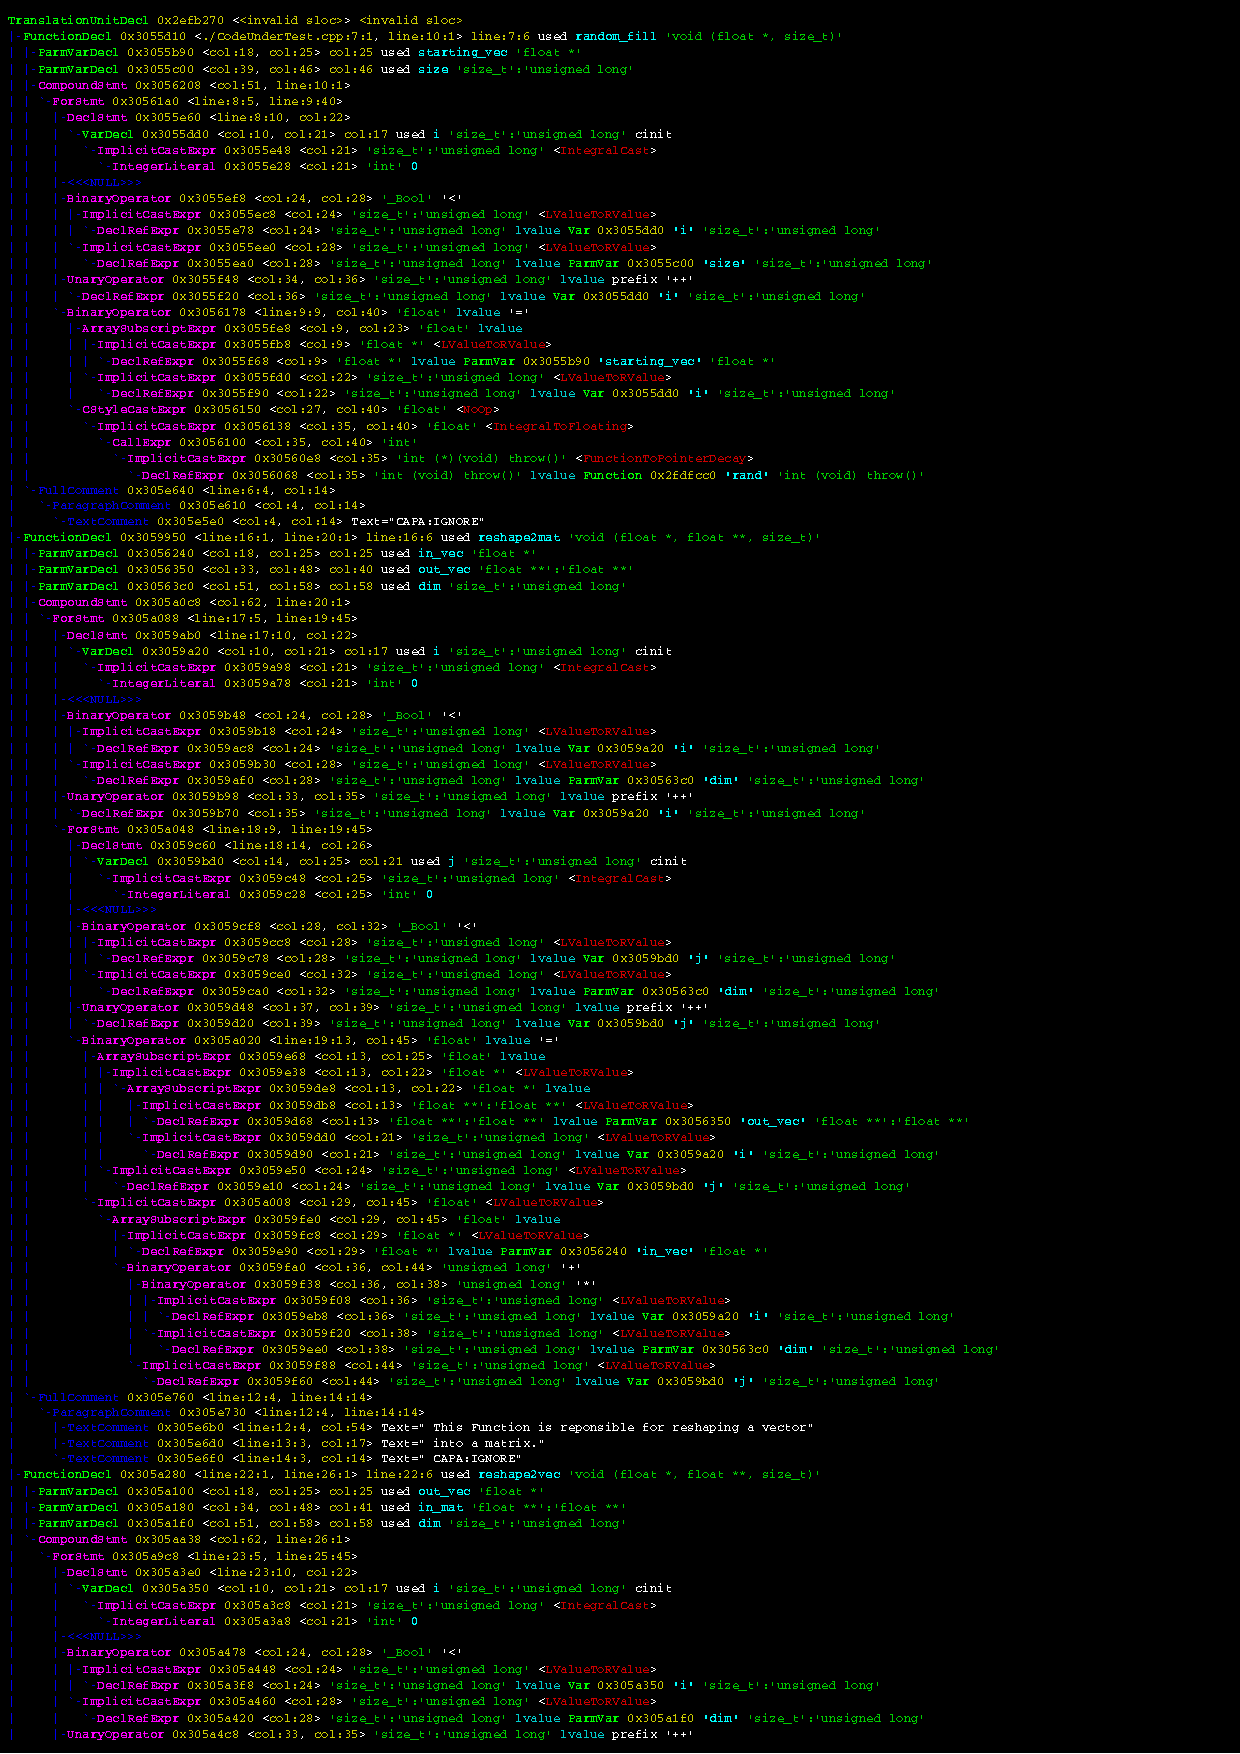
\includepdf[scale=0.8,offset=0 -45,pages=1,pagecommand=\subsection{Clang AST - Case Study}\label{AST}]{./Misc/AST.pdf}
\includepdf[scale=0.8,pages=2-]{./Misc/AST.pdf}

\pagebreak

\bibliography{references}
\bibliographystyle{IEEEtran}
\end{document}




